
\floatstyle{plaintop}
\restylefloat{table}

\newcommand{\FigQueryTime}{
\begin{figure}
    \centering
    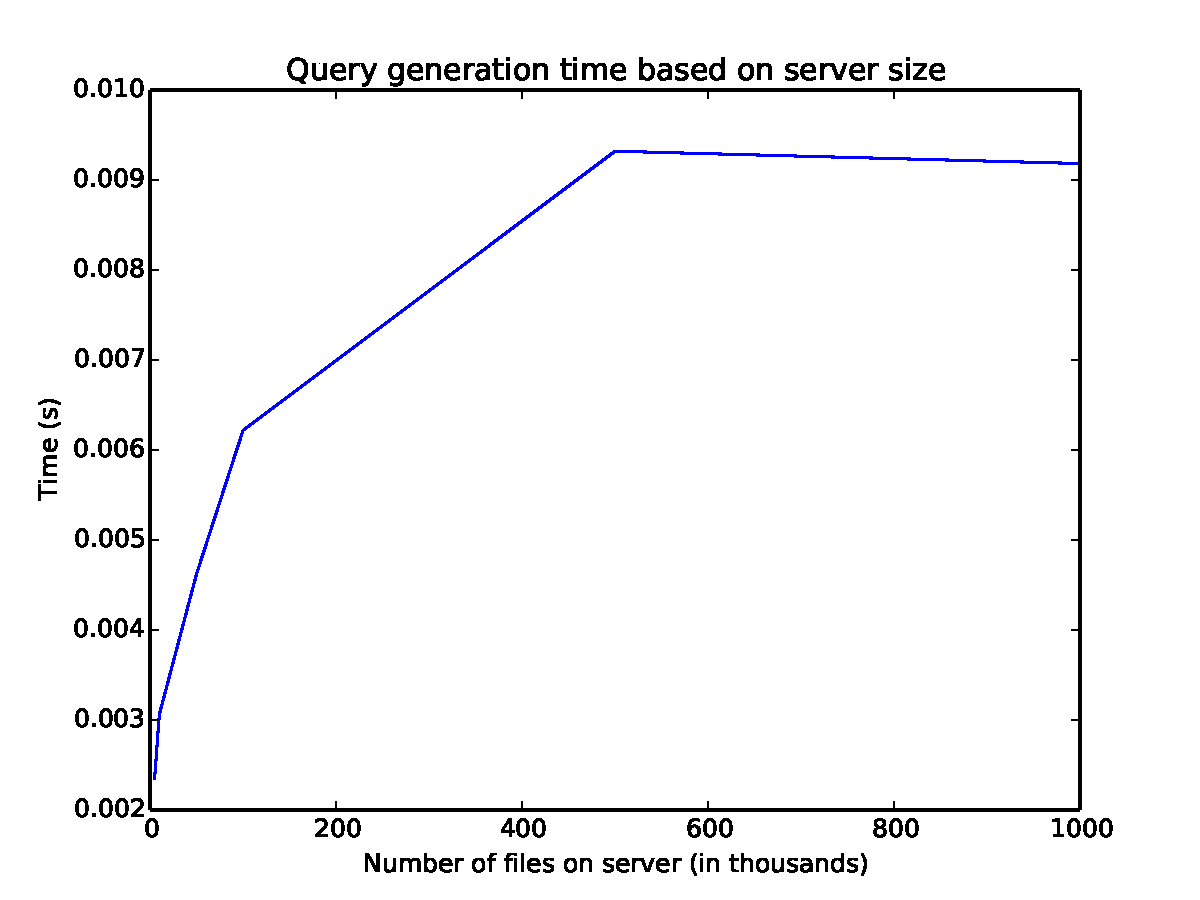
\includegraphics[width=\linewidth]{figs/QueryGenTime}
    \caption{The amount of time taken for the client to generate enough
    queries to privately ask the server for a single file.}
    \label{fig:querygentime}
\end{figure}
}

\newcommand{\FigReplyTime}{
\begin{figure}
    \centering
    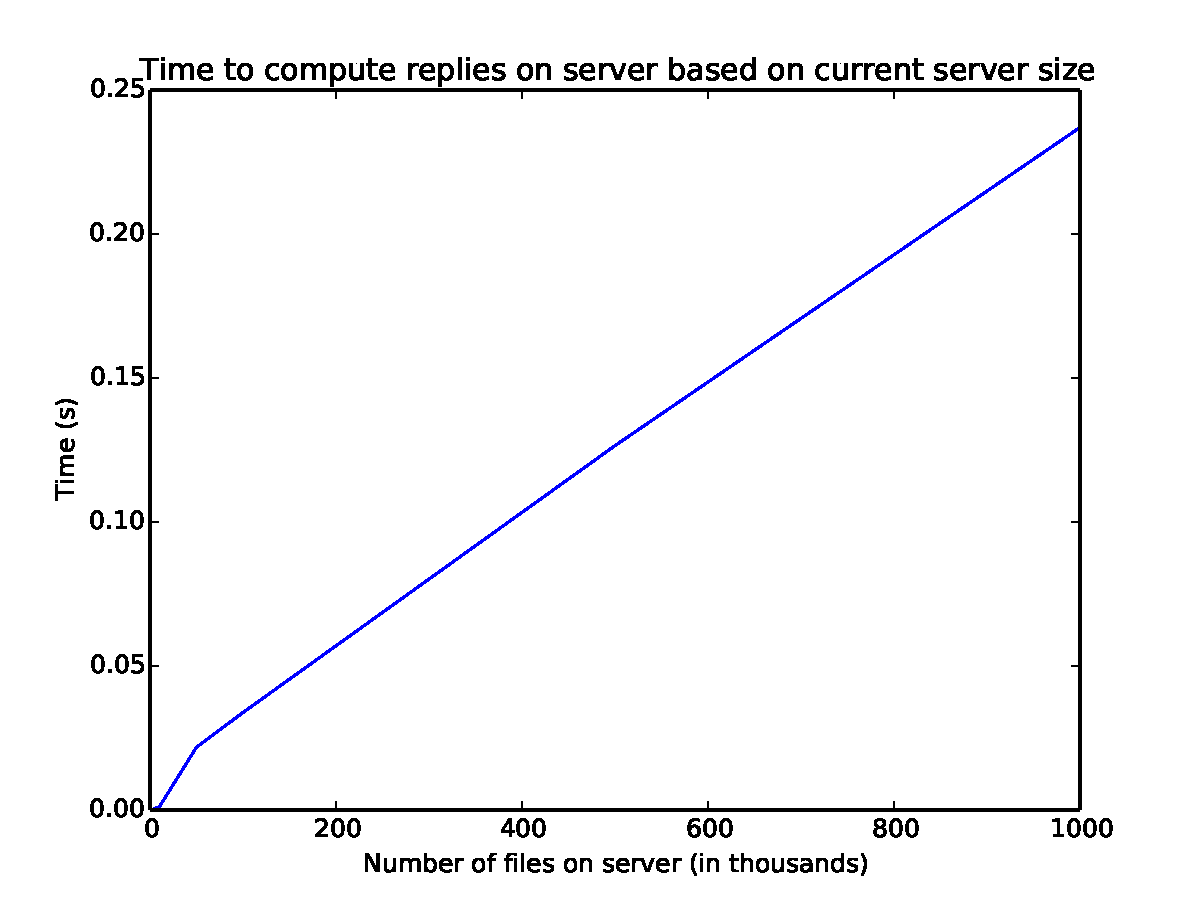
\includegraphics[width=\linewidth]{figs/ReplyTime}
    \caption{Amount of time taken for server to compute the replies to queries
    sent by client}
    \label{fig:replyTime}
\end{figure}
}

\newcommand{\FigExtractTime}{
\begin{figure}
    \centering
    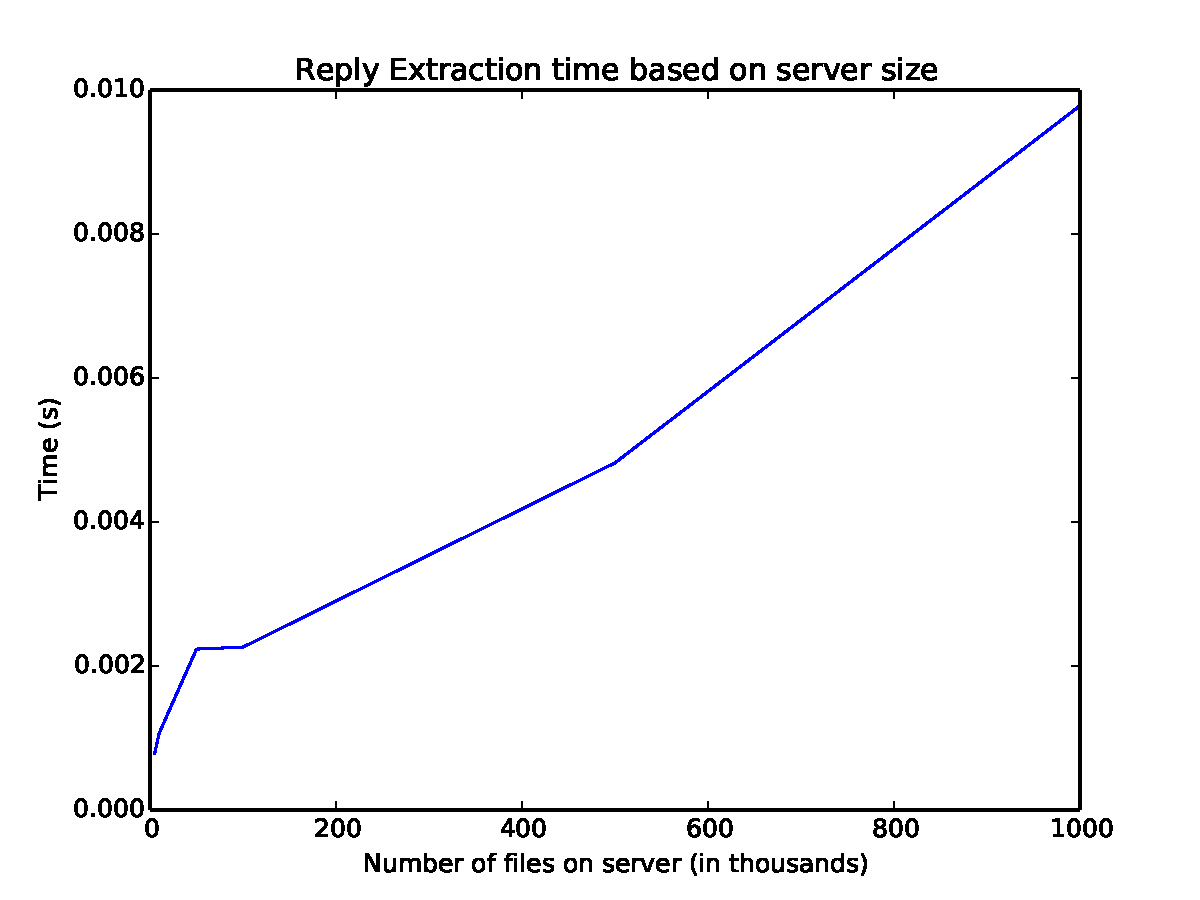
\includegraphics[width=\linewidth]{figs/ReplyExtractTime}
    \caption{Amount of time taken for the client to extract response
    from replies
    provided by the server}
    \label{fig:replyextracttime}
\end{figure}
}

\newcommand{\FigAllTimes}{
\begin{figure}[ht]
    \centering
    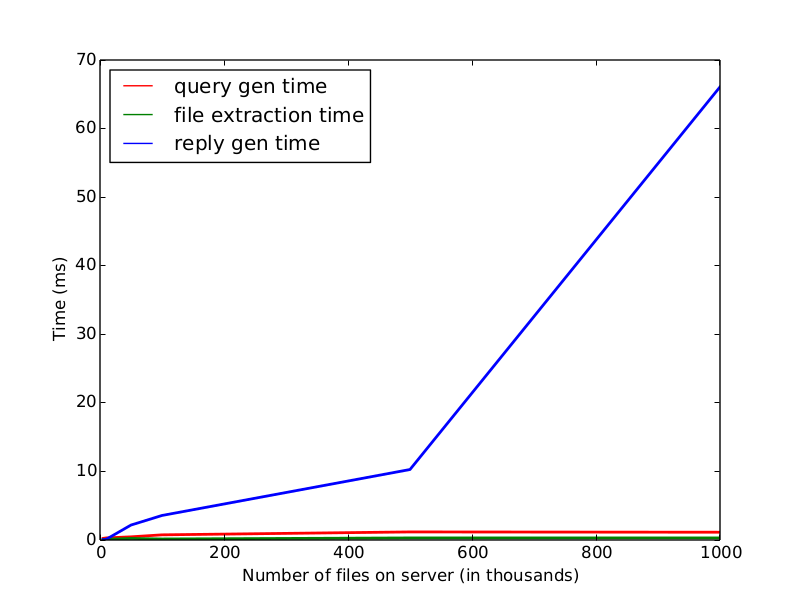
\includegraphics[width=0.7\linewidth]{figs/QueryReplyExtractOneAxisNet}
    \caption{Amount of time taken for the actions necessary for our tool to
    work. The time taken for the client to generate queries, and to extract the
    response from the server replies is very minimal compared to the amount of
    time that is spent by the server generating the replies to send back to the
    server. This time however can be decreased by using servers with hardware
    specifically designed to do these computations.}
    \label{fig:queryreplyextracttime}
\end{figure}
}

\newcommand{\FigPIR}{
\begin{figure}[ht]
    \centering
    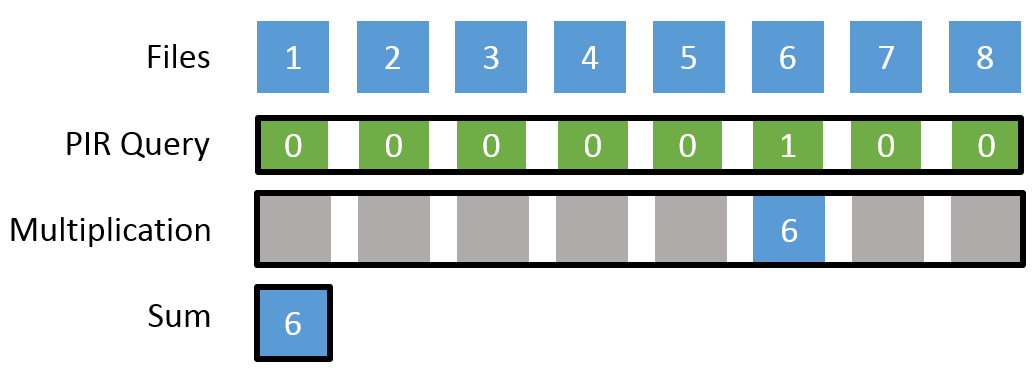
\includegraphics[width=.8\linewidth]{figs/pir-basic.png}
    \caption{\textbf{Vector-Matrix PIR}\,---\, Private Information Retrieval
    involves a client making
    a query against a database. In Vector-Matrix PIR the client encrypts a vector of  query elements and the server then multiplies the query elements
    against the database blocks homomorphically, using homomorphic addition to produce a single sum.
    This results in an encrypted value corresponding to the element where the client encrypted 1
    (instead of 0), which is sent back to the client for decryption.}
    \label{fig:pir}
\end{figure}
}


\newcommand{\FigTicket}{
\begin{figure}[ht]
    \centering
    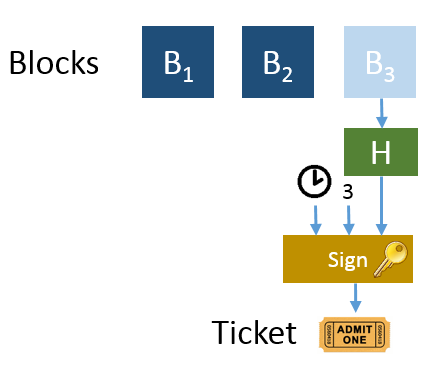
\includegraphics[width=.5\linewidth]{figs/ticket-small.png}
    \caption{\textbf{Ticket Creation}\,---\, When a file is uploaded, the server produces
            a signed ticket that commits the server to storing the block of data. The server
            signs a timestamp, the index where the data is stored, and a hash of the data, and
            returns this to the client for local storage.}
    \label{fig:ticket}
\end{figure}
}


\newcommand{\FigProof}{
\begin{figure}[ht]
    \centering
    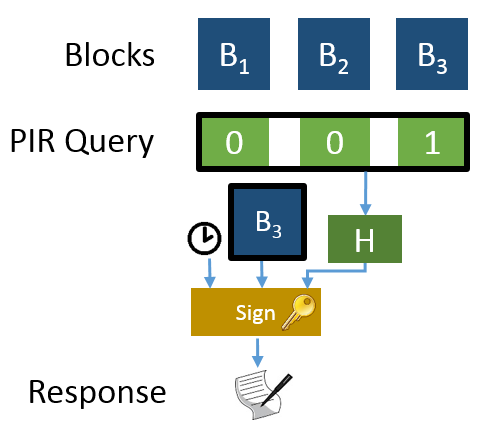
\includegraphics[width=.5\linewidth]{figs/query-small.png}
    \caption{\textbf{Proof of Censorship}\,---\, To verify a file is still in place, a client
            constructs a PIR query for its block. The
            server, without knowing which block was requested, signs the encrypted PIR query and the
            response it produces. The client decrypts the response, and can verify the data is
            correct. If it is not, the client can combine the signed response, the parameters it used
            to generate the PIR query, and the original
    ticket for this file to produce a stand-alone proof-of-censorship that can be verified by a third
    party.}
    \label{fig:proof}
\end{figure}
}


\newcommand{\TabSizes}{
\begin{table}
\centering
\begin{tabular}{l|c|c|c}
            \hline
            & Size & Generation time  (std-dev)& Validation time (std-dev)\\
            \hline

        Ticket & 120 bytes & 334 {\textmu}s (0.53) & 381 {\textmu}s (4.61)\\
        Query  & 3.8 Mbytes & 28 ms (0.44) & n/a \\
        Reply/Proof\ \  & 2.0 Mbytes & 2.8 s (0.19) & 52 ms (0.54) \\
\end{tabular}
\caption{\textbf{Ticket and Proof Size}\,---\, We implemented a prototype of our proof-of-censorship
system, simulating a database of 1~million 256-byte messages. We are able to
keep a constant size of our proof at 2 MB. This allows clients that receive a
proof of censorship to be able to easily distribute it.}
\label{tab:size}
\end{table}
}

\newcommand{\TabNumQueries}{
\begin{table}[ht]
\centering
\begin{tabular}{c|c|c|c|c|c|c|c|c}
        \hline
        Number of files    & 5k     & 10k    & 50k     & 100k   & 500k   & 1M 
        & 10M  & 100M\\
        \hline

        Recursion depth    &  1     &  1     &  2      &  2     &   2    &   3 
        & 3  & 3\\
        Aggregation value  & 300    & 420    & 96      & 64     & 126    &  16
        & 16 & 15\\

        Query size (MBytes)    & 0.53 & 0.75 & 1.44 & 2.5  & 3.9  & 3.8 & 8.0  &
        17.7 \\

        Reply size (MBytes)    & 0.56 & 0.78 & 1.44  & 1.0  & 2.0  & 2.0
         & 2.0  & 2.4 \\
\end{tabular}
\caption{\textbf{Small File Scaling}\,---\, We measured query and response sizes
    generated for several different database sizes with 256~byte files to determine
    how the system scales for a Twitter-like content server. We find that even at millions
    of files, the system remains
    relatively practical: an 8~MByte query and 2~MByte response are needed to select
    a single file privately (with accompanying proof of censorship) from 10~million files.}
\label{tab:numQueries}
\end{table}
}

\newcommand{\TabNumMBQueries}{
\begin{table}[ht]
\centering
\begin{tabular}{c|c|c|c|c|c|c|c|c}
        \hline
        Number of files    & 5k      & 10k    & 50k     & 100k   & 500k   & 1M 
        & 10M  & 100M\\
        \hline

        Recursion depth    &  2      &  2     &  2      &  2     &   2    &   2 
        & 3  & 3\\
        Aggregation value  & 1       & 1      & 1      & 1      & 1       &  1
        & 1 & 1\\

        Query size (MBytes)    & 17.8  & 25.0 & 14.0 & 19.8 & 44.2 &
        62.5 & 121.3 & 174.1 \\

        Reply size (MBytes)    & 32.8  & 32.8  & 73.1  & 73.1  & 83.7  &
        83.7  & 138.4  & 199.4 \\
        % Bits of Security & 209 & 209 & 248 & 248 & 248 & 248 & 90 & 209\\
        % Polynomial Degree & 4096 & 4096 & 2048 & 2048 & 2048 & 2048 & 4096 &
        % 4096\\
        % Modulus Bits & 60 & 120& 60 & 60 & 60 & 60 & 180 & 120\\
\end{tabular}
\caption{\textbf{Large file scaling}\,---\, We also measured query and response sizes
        assuming 1~MByte files, to approximate our system being applied to an image or video-streaming
        content server. The XPIR optimizer chooses different security,
        polynomial and modulus parameters for each database size for 1~MByte
        files, due to it attempting to limit the amount of data the client
        has to send and receive over the network. While the parameters that
        are chosen are not always the most secure or privacy preserving,
        these parameters do result in the least amount of bandwidth
        necessary for clients to use. Additionally, while overheads are low,
        even with only 50
        thousand files
        in a database, responses are 73~MBytes for a single megabyte file, likely making application of
        proof of censorship impractical to video streaming content providers.}
\label{tab:numMBQueries}
\end{table}
}

%\widowpenalty1
%\clubpenalty1
\newcommand{\imm}[1]{\textcolor{blue}{IMM:#1}}
\newcommand{\ewust}[1]{\textcolor{green}{ewust:#1}}
\newcommand{\tim}[1]{\textcolor{red}{TIM:#1}}

\chapter{Proof of Censorship: Enabling centralized censorship-resistant content providers}\label{ch:poc}
%\setlength{\belowcaptionskip}{0pt}
%\setlength{\floatsep}{0pt}

% \author{Ian Martiny\inst{1} \and Ian Miers
% \inst{2} \and Eric Wustrow\inst{1}}
% \institute{University of Colorado\\
% \email{\{ian.martiny,ewust\}@colorado.edu} \and Johns Hopkins University\\
% \email{imiers@cs.jhu.edu}}
% %\author{Anonymized for Review}
% %\institute{}

% \maketitle

% \begin{abstract}

% Content providers often face legal or economic pressures to censor or remove
% objectionable or infringing content they host. While decentralized providers can
% enable censorship-resistant storage, centralized content providers remain
% popular for performance and usability reasons. But centralized content providers
% can always choose not to respond to requests for a specific file, making it difficult
% to prevent censorship. If it is not possible
% to prevent, is it possible to detect and punish censorship on a centralized
% service?

% A natural approach is to periodically audit the service provider by downloading
% the file. However, failure to download a file is not a proof of censorship.
% First, the provider could claim benign failure. Second, the proof is
% non-transferable: verifying censorship requires third parties to individually
% request the censored file.  Moreover, a content provider may only selectively
% deny access to particular users or only for a short time frame. As such,
% checking by downloading does not work even for third parties who are online and
% willing to make queries.

% % A related line of work studies Proofs of Retrievability~\cite{JulesPOR}, studies the pr

% % Proofs of retrievability~\cite{JulesPOR} were proposed to solve similar problem: ensuring that a potentially malicious content provider does not delete an outsourced file. A natural approach is to periodically download the the file from the provider as a way of auditing it. However, failure to download is not a transferable proof of censorship. In particular, while a 


% % %of retrievability have been proposed which allow content providers to prove they
% % still have the data of a previously uploaded file. However, a provider that
% % wishes to remove a file can simply ignore or stall requests for it, rendering
% % the proof of retrievability inconclusive. While auditors may catch this
% % behavior, there is no transferable proof that a content provider is selectively
% % censoring a file, meaning offline third parties cannot verify an auditor's claim
% % of a removed file.  In addition, the provider can restore a previously-censored
% % file without any lingering evidence of the temporary removal.

% In this paper, we introduce
% \emph{proof of censorship}, whereby a content provider cannot delete or
% otherwise selectively remove content from their service without
%  creating transferable cryptographic proof of their misdeed. Even if the
% provider restores the file at a later date, the proof remains valid, allowing
% the reputation of a content provider's commitment to censorship resistance to be
% based on the existence (or absence) of such proofs.

% \end{abstract}

\section{Introduction}

Online censorship is done in many ways. In addition to blocking access to
websites, censors also use legal means to remove information from content
providers directly, such as through laws like the DMCA~\cite{dmca} in the United States.
In the second half of 2016, Twitter received
over 5,000 removal requests from government and police agencies worldwide, and
complied with 19\% of them~\cite{twitter-transparency}. In one example from August 2016, Twitter complied with
a Brazilian government request to remove a tweet comparing then-mayoral
candidate Rafael Greca to a fictional villain from the 1992 film Batman
Returns~\cite{twitter-rafael-greca}.
% https://www.lumendatabase.org/notices/12866354

This style of censorship can be significantly less apparent than overt website
blocking.  Because the service remains accessible, users are unaware of the
content that may be secretly withheld from them. While some content providers
(including Twitter) publish transparency reports containing overall statistics
or examples of removed
content~\cite{twitter-transparency,facebook-transparency,google-transparency},
these reports are difficult to confirm or refute: How can users know if the
transparency reports themselves have not been similarly censored?

While decentralized or distributed tools provide a way to make content robust
against censorship, these techniques do not fully solve the problem. In a
distributed censorship-resistant scheme, users must download and use specialized
software which may itself be blocked by a censor. Due to this requirement,
these tools are only utilized by well-informed users, while the majority of
people rely exclusively on centralized content providers. Thus, there are clear
advantages to providing censorship resistance in a centralized content storage
context.

One idea proposed to incentivize censorship-resistant content
providers to not delete data  is to use \emph{proof of retrievability} (PoR) to enable content providers
to prove that they still retain a copy of a file. In PoR, providers respond to
requests or challenges for specific subsets of a file they have agreed to store.
A provider responds with the subset, proving (over many challenges) that they
likely still store the entire contents of the file. With enough successful PoR
challenge responses, a client can reconstruct the file, meaning that a provider
that gives valid PoR responses for a file necessarily provides access to it.
While this is a useful starting point, there are two major problems with this approach.

% ewust: we detail the two problems in the next paras...maybe we could merge this sentence in though?
%proving a positive that a client has a file is not sufficient to prove a negative, that a provider has never denied access to that file.

First, the content provider can always choose to not respond to a PoR request.
Note that this is different from providing an invalid response to a request. By
simply leaving a connection open and providing no response, the service never
provides any incriminating evidence that they are not providing access to the
file. While other clients can see this suspicious behavior, the provider could
choose to respond correctly to some subset of users, seeding confusion
and distrust over claims of censorship.

Second, the content provider can cease this behavior at any time, with no
evidence that they ever censored a file. For example, a provider could wait
until a certain number of users realized a file was removed or journalists started
to ask questions before they reverted the decision to censor a file. Such a
provider could pretend they never censored a file, and those that observed that they
did would have no transferable proof. This allows a provider to censor
files at will, and restore them only when convenient.


% Third, just because a file is retrievable does not, in actual fact, mean it can be retrieved.  Proofs of retrievability 
% %Proof of retrievability/proof of storage is one idea to accomplish this, but
% %has a couple drawbacks:
% %1. provider can choose to not respond to proofs
% %2. provider can always restore a file to rid evidence of previous censor
% %

\medskip

%We propose a transferable proof of censorship that provides a cryptographic
%proof when a provider censors.
In this paper, we describe a way that a content provider can be held accountable
for the files that they censor. We do this via a \emph{proof of censorship} that
a content provider unavoidably produces should they censor a file. Furthermore,
these proofs are transferable, meaning that once one has been produced, others
can verify the cryptographic proof and see that it attests to a censored file.
Even if the content provider restores the original file, this proof still
maintains the evidence of previous censorship.

%We accomplish this by leveraging a simple addition to private information retrieval
%to hide what information we are requesting from the provider, while having it
%sign the information provided.
To construct our proof of censorship, we use
private information retrieval (PIR) which hides what information a client is
requesting from a server. At a high level, servers commit to storing (encrypted)
files by signing hashes of those files on upload. To download a file, a client
performs a PIR query, which the server responds to, signing both the PIR query
and the server's response. Because the server does not know what file a client
is requesting, it cannot selectively answer queries. To censor a file, the
provider must return garbage data. Upon decryption of the PIR response, the
client can confirm the file has been censored, and can reveal its PIR queries
and the signed response to the world. Anyone with this proof (and the content
provider's long-term public key) can verify that the content provider has
removed the file.


Our proofs of censorship are compact and relatively efficient to verify: in the
event of censorship, for a reasonable size database, the proof is on the order
of a few megabytes, and takes approximately 50 milliseconds to verify on a laptop
computer.


%Our contributions are:
%-proof of censorship concept
%-design and implmentation of a robust proof of censorship
%-proof of correctness?
%
%Section TK has stuff in it.

\section{Background}

\FigPIR

To describe our proof of censorship, we first provide background on private
information retrieval (PIR)~\cite{pir}. PIR allows a client to request data from a server
without revealing to the server what data is being requested. A naive way to
accomplish this is for the client to download the entire database from the
server, then select its data locally. This method is bandwidth inefficient,
however, and does not scale to large datasets.

There are two settings for PIR. In \emph{information-theoretic} PIR (ITPIR), a
set of $N$ servers share the database, with clients making requests to all of
them and combining their responses to obtain the requested files. If at least
one of the servers is not colluding with the others, the client's request
remains private. In \emph{computational} PIR (CPIR), a single server stores the
database, and clients use homomorphic-encrypted requests to retrieve data. As
long as the computational hardness assumptions on the underlying cryptography
hold, the server cannot determine what information the client requested. As we
are focused on a single centralized content provider, in this paper, we only
consider and describe CPIR.

Many CPIR schemes fall into the ``matrix-vector'' 
model~\cite{cryptoeprint:2017:825}, which is illustrated in 
Figure~\ref{fig:pir}. In this model, CPIR uses a (IND-CPA-Secure, additive)
homomorphic encryption that allows operations done on ciphertext to correspond
to operations done on the corresponding plaintext. As an example, consider an
additively homomorphic encryption function $E()$ with corresponding decryption
function $D()$  that allows addition of ciphertext  and multiplication by a
constant; i.e,:

$$D(E(a) + E(b)) = a + b$$

\noindent and $$D(E(a)\cdot c)=a\cdot c.$$


To perform a PIR query, a client constructs a vector of encrypted 0s and 1s. For
example, if the server has $n$ blocks, and the client wishes to retrieve block $x$ 
from the server where  $0 \leq x < n$ , the client sends a query vector $Q$ to
the server, comprised of $q_{i \neq x} = E(0)$, and $q_x = E(1)$. Note
that the IND-CPA security of the encryption scheme implies that the server
cannot determine which $q_i$ is the encryption of 1.

With $Q$, the server (homomorphically) multiplies each $q_i$ with its
corresponding data block $d_i$ in the database. The server then takes the
homomorphic sum over the result. When $i \neq x$, the multiplication by $E(0)$
will ensure the corresponding block does not contribute to the later-decrypted
sum. The response is sent back to and decrypted by the client,
resulting in $D(\sum_i q_i\cdot d_i) = D(E(1)\cdot d_x) = 1 \cdot d_x$.

The PIR library that we use (XPIR~\cite{xpir}) provides two optimizations:
recursion and aggregation. Recursion allows
clients to send fewer query elements to the server, by breaking the database into
a $d$-dimensional cube, and having the query select the row/column vectors.
For example with a database of 100 records, it can be broken into a $10\times
10$ table of elements. The client sends 10 queries, which the server copies and
applies to each row effectively selecting a singular column. Then, a separate 10
queries can be used to select a single element from that column. Thus the client
sends a total of 20 query elements, as opposed to 100 (with no recursion).

Aggregation allows a client and server to pack multiple plaintext files into a
single element. For example, if the ciphertext allows for an absorption of
768~bytes, but files are only 128~bytes, the database could utilize aggregation,
fitting 6 files into each block. Clients then select the block of 6 files that
contains their requested file, and locally discard the other 5.
With aggregation, the client sends fewer request elements to the server, resulting in
smaller queries.


\section{Threat Model}

We consider a setting consisting of a single centralized content provider with
multiple clients who upload and download content.  Clients upload files to the
provider, and distribute tickets that enable others to download the file. The
information in a ticket can be summarized in a URL to be provided to others.
This allows clients to easily share tickets in the same way they would
distribute online content to others. In this model, we wish to detect a
censoring content provider while preventing malicious clients from making false
accusations. We achieve two properties:

\begin{description}
	\item[Non-repudiation of Targeted Censorship] A provider cannot
	selectively censor a file while responding to queries from honest clients
    without producing a transferable proof of their misdeed.
	\item[Unforgeability] Against a non-censoring content provider, an attacker
             cannot  forge a proof that a file was  censored.
\end{description}

We note that our threat model does not  prohibit a provider that chooses to delete
or remove access to all of its files: a provider can always shut down entirely,
or refuse to sign statements with its private key.


\section{System Design}

In this section, we describe the details of our proof of censorship. A proof of
censorship has two parts: a commitment from the server that it will store and
distribute a file, and second, a later proof that it failed to uphold that
commitment. The first part is obtained during file upload, where the server
returns a signed and timestamped \emph{ticket} that efficiently represents the
commitment to store the file, while the second part is obtained when a
client downloads the file the server is attempting to censor. We assume the
server has a widely published long-term public signing key.

We begin our description assuming that a file fits in a single block that can be
requested in a single PIR query to the server. In
Section~\ref{sec:poc-multi-block}, we describe how to efficiently extend this idea
to provide proofs of censorship for files that span multiple blocks.

\subsection{Proof of Censorship Construction}\label{ssec:POC-construction}

\FigTicket

\paragraph{Ticket Construction}
On upload, a client will upload an encrypted block that represents
the file. The server chooses an index for the block to be stored, and provides
a signature over the data and the index. For block data $B_i$ stored at index
$i$, the server hashes the block data to obtain $H(B_i)$. The server then signs
the tuple containing a timestamp $t$, the index $i$, and the block hash $H(B_i)$
using its long-term private key. This signature, along with $t$, $i$, and
$H(B_i)$ are sent to the client in the form of a \emph{ticket}.

This ticket can be encoded into a URL that can be distributed easily to other
users in the form of:
\begin{center}
    \texttt{https://<service>/\#$H(B_i)$/$i$/$t$/$sig$}
\end{center}
where $sig$ is the server's signature of the ticket. This gives the client all
of the information it needs to verify as well as a simple way to distribute the
ticket. Additionally the sensitive information is provided to the client in such
a manner that it is not passed to the server, as values after a \# symbol are
only handled locally in browsers.

The client then verifies that the ticket is well formed and valid. First, the
client hashes the data it has uploaded to obtain $H(B)$. Then, it ensures that
the timestamp $t$ it received from the server is a recent
timestamp\footnote{The client must ensure $t$ is not located days
in the future to avoid a server producing invalid proofs later.}.
Finally, the client checks the signature of the ticket, using
$t$, $i$, and the client-computed $H(B)$. If the signature is valid, the client
stores the ticket for this block. If any checks fail, the client can attempt to
re-upload their file until they receive a well-formed ticket.
Figure~\ref{fig:ticket} illustrates how tickets are generated during file
upload.


%associated
%with the file. The server will provide a signature over these blocks, committing
%to pairs of their hashes and the index where they will be stored. For each
%block data $B_i$ stored at index $i$, the server hashes the index with the
%block data. The server arranges these hashes ordered by index into a Merkle
%Tree, obtaining the Merkle Root hash $H$. The server then signs $H$ along with a
%timestamp using its long-term identity key to produce a \emph{ticket}. The
%ticket is sent to the client, along with the indexes associated with each block.
%The client reconstructs the Merkle Root hash $H$ itself locally, and verifies
%the signature from the server to ensure the ticket is valid.


\FigProof

\paragraph{File Download}
To download a file, a client creates a PIR query that will
result in a proof of censorship if it does not receive the file requested.
During a normal PIR request, a client encrypts a vector of 0 and 1 elements
using using random coins for the encryption. In our scheme, these coins are the
output of a pseudorandom generator  with a \emph{seed} ($Q_{seed}$) randomly
selected by the client. This allows us to later reproduce the same query with
only the seed and the index $i$. With this we create a compressed representation
of the query which consists of the queried index (in the clear), and the seed.

The client creates the request $Q$ and sends it to the server, along with 
the public key (as well as any
cryptographic parameters needed to allow the server to perform homomorphic
operations on the query\footnote{E.g. in Paillier, this involves the public
modulus generated by the client.}). The server then performs the query over its
database using PIR, producing a short reply $R$ that contains an encrypted
representation of $B_i$. The server then hashes $Q$ (including the public key) to obtain $H(Q)$, and
produces a signature over a timestamp $t$, the query hash $H(Q)$, and the reply
$R$. The server sends this signature, along with $t$ and $R$ to the client.

The client then extracts $B_i$ from $R$ using standard PIR extraction (i.e.
decrypting $R$ with its $Q_{seed}$-derived private key). The client then checks if this is the
expected file by comparing it to the hash in the corresponding ticket for this
file.
If the client detects that the block has been censored, it now has a proof of
censorship in the form of the server's response. The client publishes the
original ticket, the server's signed PIR reply, and its $Q_{seed}$ as a proof of
censorship.

%Note that the ticket does not have to be published by or even known
%to the same party that receives the proof, meaning this could be stored by
%another client and combined later.

During this process, the server does not know what file is being
requested. Therefore, to censor a file, the server must either not respond to
any queries, or risk revealing that it has removed a file from its database.

\paragraph{Verifying Proofs of Censorship}
Given the server's public key, a signed ticket, a signed reply, and a query
seed, a third
party can verify whether the proof is valid evidence of censorship. To verify a
proof of censorship, a verifier must perform several steps, detailed below.

\begin{enumerate}
\item \textbf{Check Timestamps} The verifier checks that the ticket's timestamp
        ($t_t$)
        is before the reply's timestamp ($t_r$), ensuring that the query took
        place after the server committed to storing the file.
\item \textbf{Check Ticket Signature} Given the ticket's timestamp $t_t$, the
        requested index $i$, and the hash of the file $H(B_i)$, the verifier
        validates the ticket's signature with the server's public key.
\item \textbf{Regenerate PIR Query} Verifier uses $Q_{seed}$ and the index $i$
        to deterministically derive the PIR query $Q$, and computes the hash
        over the query $H(Q)$.
%\item \textbf{Check query hash} The verifier hashes the generated query $Q$ to
%        obtain $H(Q)$, and checks that this matches the query hash provided in
%        the server's reply.
\item \textbf{Check Reply Signature} Given the reply's timestamp $t_r$, the
        computed hash $H(Q)$, and the server's reply, the verifier checks the
        reply's signature using the server's public key.
\item \textbf{Extract Reply} Again using the key derived from $Q_{seed}$, the
        client extracts the PIR reply $R$ to obtain $B_i$.
\item \textbf{Check Data Hash} The verifier finally compares the hash of the
        extracted data $B_i$ to the hash committed to in the ticket. If the
        hashes are equal, the server did \emph{not} censor the file, and
        returned the expected result. However, if the hashes do not match, this
        is a valid proof of censorship.
\end{enumerate}



\subsection{Handling Multiple Blocks}
\label{sec:poc-multi-block}

%\imm{The point here is to prevent having to include every block in the proof of censorship}
So far, we have described how a client can efficiently receive a proof of
censorship for a single uploaded block, but this does not address what happens
if a file is larger than a single block. While a client could easily split up a
file into multiple blocks, and receive a ticket for each block, storing each of
these signed tickets may be expensive.

Instead, we can extend our design to allow for multiple blocks to receive a
single ticket, while still allowing a proof to catch if an individual block is
censored. To do this, our ticket will contain a Merkle tree root~\cite{merkle}
in place of the single block's hash. The leaves of the Merkle tree will be the
hashes of each block's data, and the ticket will consist of the list of hashes,
and the final signature over the Merkle root, timestamp, and block index
range.

% Note: these hashes are still stored somewhere...so does this save anything?
To verify a proof, the verifier reconstructs the Merkle root from the
suspected censored block and its Merkle tree-adjacent neighbors, and uses the
root to verify the ticket. Thus, a
verifier does not have to know all of the hashes of the tree, but rather only
those that allow it to reconstruct the Merkle root ($log(N)$ hashes for an
$N$-block file). This allows proofs to stay relatively compact even as the file
size grows. After validation of the ticket, the verifier can be assured that the
hash of the suspected block ($H(B_i)$) they have been given is the correct hash
for the given block $B_i$, and can perform the remaining checks described
previously.

\subsection{Security Argument}

\subsubsection{Non-repudiation}
Assuming an honest client, that $H$ is a collision resistant hash function,
and the query privacy of the PIR scheme, we can show
that the non-repudiation property holds (that a selectively censoring server
will produce a proof of censorship).

The server can attempt to censor a file in two ways: by not responding to
queries for the file, or by creating a malformed response. Malformed responses
themselves can be made by either changing the data as it is stored/responded to,
or by creating invalid signatures over the reply depending on the query.

A server that chooses to change its response based on the query (either not
respond or produce an invalid signature) is prevented by the privacy of the PIR
scheme. The server cannot know what file is being requested, and thus cannot
selectively perform different behaviors based on the file requested. Honest
clients will detect and reject malformed responses, effectively censoring the
file they requested without the server knowing which file it is censoring.

The server can modify a file block directly, but because they have
committed to the hash of the block's data in the ticket, and because of the
collision resistance of the hash, the server is unable to change this data
without producing a proof when that data is next requested.

\subsubsection{Unforgeability}

We show that the scheme is unforgeable assuming the servers signature scheme is
unforgeable, $H$ a  random oracle, and the PIR scheme is the ``vector-matrix
type''~\cite{cryptoeprint:2017:825} with an underling encryption scheme that  is
``homomorphic quasi-committing.''

\paragraph{Homomorphic Quasi-committing}
A homomorphic encryption scheme $gen,enc,dec$ is homomorphic quasi-committing if
an attacker cannot produce a ciphertext $ct$ and values
$m_1,m_2,c_1,\allowbreak c_2,pk,sk,r_{keygen},r_1,r_2,$  such that $$pk,sk\leftarrow
gen(\lambda;r_{keygen})$$ $$ct=c_1\cdot enc(pk,m_1;r_1)+c_2\cdot
enc(pk,m_2;r_2)$$ where $$dec(sk,ct)\ne c_1\cdot m_1+c_2\cdot m_2 $$

This property is closely  related to  correctness, which states that for all
choices of random coins and query indexes, an incorrect result is returned with
negligible probability. However, crucially,  correctness is insufficient here.
First, it does not ensure that a given query could be correct for two different
choices of coins (and therefore private keys) and query indexes. I.e, it doesn't
explicitly prevent a forgery where an attacker opens a legitimate query to a
different result. Second, correctness effectively says there is a negligibly
set of bad random coins which cause the scheme to fail. It provides no
protections against an attacker choosing from that subset intentionally.

Homomorphic quasi-committing is a strong property to require of an encryption
scheme. For the rest of the paper, we assume that the underlying encryption
scheme used in the PIR is homomorphic quasi-committing in the random oracle
model where $r_{keygen},r_1,r_2$ are the output of a random oracle $h$ evaluated
on a nonce $nonce$ and the query index $i$.

Consider an attacker interacting with an honest content provider who produces a
ticket and a proof of forgery for that ticket. Either the ticket or the PIR
transcript must be forged.  Forgeries in the ticket are prevented by the
collision resistance of $h$ and the security of the signature scheme.

\paragraph{Security Argument} 

We now consider the case of forgeries in the PIR transcript.  By the collision
resistance of the hash function and security of the signature scheme, a attacker
cannot substitute  either the query or response. As such the PIR transcript
itself must represent the actual query to and response from the provider. The
only freedom an attacker has here is the choice of openings for the transcript
(i.e. the random coins used for encryption and the public and private keys.) and
she must reveal those as part of the proof. Thus the attacker reveals
$$pk,sk,r_{keygen},r_1,\ldots,r_n,ct$$ for a query on block $i$ such that
$$ct=B_i\cdot enc(pk,1;r_i) + \sum_{j=0,j\ne i}^{N}  B_j\cdot enc(pk,0;r_j) $$
and $$dec(sk,ct) \ne B_i$$ It follows that $0,1,\sum B_j,\allowbreak
B_i,pk,sk,r_{keygen}, \sum r_j ,r_i$ violates the `homomorphic quasi-committing''
property of the encryption scheme for $B_*= \sum_{j=0,j\ne i}^{N}  B_j\cdot
enc(pk,0;r_j)$ By assumption, this is not possible.
%
%openings for the transcript (i.e. the random coins used for encryption and the public and
% private keys) which she must reveal as part of the proof. The attacker may
% choose to deviate from the protocol to generate a malformed
% query $Q$, such as by choosing a different public key, different random coins,
% or encrypting something besides the 0s and single 1 required to query the single
% block $i$. However, the hash of $Q$ has been committed to by the server, and is
% regenerated by the verifier. Even in the event that the attacker manages to
% construct an invalid query, it must be byte-wise equivalent to a valid one
% generated by the honest verifier (otherwise the hash of $Q$ in the signed reply
% will be invalid). Thus, the honest verifier's query would have produced the same
% reply from the server, and should be openable by the honest verifier's key.

\section{Implementation and Evaluation}

We implemented our proof of censorship construction on top of XPIR, a fast PIR
tool written in C++~\cite{xpir}. Our implementation consisted of several hundred
lines of modifications to XPIR, as well as an approximately 500-line application
using the resulting libXPIR library. We used OpenSSL to perform the necessary
signatures and hashes in our protocol.

The parameters we selected for testing were motivated by a simple text-only
Twitter-like application, where messages are short (256~bytes, enough to include
a short post and its metadata). We tested against a database of 1~million
simulated messages in order to evaluate the time and size of different parts of
the system. We used a quad-core Intel Core i5 CPU (3.30 GHz) with 32~GBytes of RAM
to evaluate our prototype.

\TabSizes

Table~\ref{tab:size} shows the size and time to generate and validate our
ticket, PIR query, and PIR reply (containing the proof). For our XPIR
parameters, we choose to use XPIR's Learning with Errors implementation with 248
bits of security, using a polynomial of degree 2048 and a modulus of 60 bits,
with recursion level ($d$) 3, and aggregation ($\alpha$) 16. All of
the client operations are relatively fast: ticket validation (395~{\textmu}s),
query generation (27~ms), plaintext extraction (3.5~ms), and proof validation (45~ms)
suggest that clients could be implemented in smartphones or even Javascript
web pages without significant performance issues~\cite{webcrypto}.

\subsection{Scalability} \label{ssec:poc-scalability}

We performed measurements of our proof of censorship
and underlying PIR library to determine how the system scales. We measured the
performance of downloading a single file with various database sizes, ranging
from 5,000 to 1~million files of both small (256~byte) and large (1~MByte) size.
For each database size, we used
XPIR's built-in optimizer to determine the best parameters. XPIR chooses between
two encryption options (Paillier, and the lattice-based learning
with errors (LWE)), varying parameters of each to be optimal given a bandwidth
estimate, file size, and number of files. We encouraged XPIR to optimize for
small query and response sizes by providing a low bandwidth. Although Paillier
produced the smallest query/responses, its
server-side processing time was many orders of magnitude slower than LWE, effectively making it
impractical. As a
compromise between bandwidth and processing time, we selected LWE encryption
optimized for small query and response sizes. For small files (256~bytes), the XPIR
optimizer selected a polynomial of degree 2048 and
60-bit modulus with varying recursion and aggregation values depending on
database size. When
considering 1~MByte files the optimizer selected differing LWE flavors, all
above the 80-bit security level, with polynomial degrees ranging from 2048 bits to
4096 bits and modulus bits ranging from 60 bits to 180 bits.
%This variance in
%larger files is due to the XPIR optimizer attempting to limit the amount of data
%the client has to send and receive.

\TabNumQueries
For each database size we measured the size of queries a client would have to
generate and the time to generate them. On the
server side we measured the amount of replies it needed to send (based on file
size and aggregation value) and the time it took to construct those queries. And
finally, back on the client side, we measured the time it took to extract the
actual response from the given replies. The results of our experiments are
shown in  Tables~\ref{tab:numQueries},~\ref{tab:numMBQueries} and
Figure~\ref{fig:queryreplyextracttime}.

\FigAllTimes
\TabNumMBQueries

For comparison, we allowed the optimizer to select
Paillier 1024, which generates a 34.7~KB query and a 9.6~KB response when
querying a 256~byte file from 1~million files.  While this is several orders of
magnitude smaller than LWE, server reply generation took nearly 2 hours for a
single query. However, query generation and extraction times on the client were
still fast (100ms and 77ms respectively).  This suggests that with specialized
modular arithmetic hardware on the centralized server, reply times could
be considerably improved, potentially making this scheme practical and very
attractive for its small query and response sizes.

%As mentioned in every case the optimizer chose the same settings for our system,
%no matter the number of files, this lead to a consistent size for our ciphertext
%(in homomorphic encryption the size of the ciphertext is often larger than the
%size of the plaintext). The size of our ciphertext was consistently 32,768
%bytes.
%
%TK: show how it scales...managed to run a 10-million message test:
%10 million files
%params : LWE:248:2048:60:15
%    d      : 2
%    alpha  : 345
%            Query: 11168 KB 73.1825 ms per query
%            Reply: 6304 KB 2670.73 ms
%            Extract: 256 bytes 11.0772 ms
%            Proof: 124.839 ms
%

We also note that a server need not contain all of its files in a single
PIR database. Instead, one could partition the file space into many buckets, and
requests could be made over a much smaller number of files in each bucket,
similar to an idea proposed in bbPIR~\cite{bbPIR}. This
allows for a tradeoff between the granularity at which a server can censor
without producing a proof, and the efficiency or scalability of the system as a
whole. With more buckets, a server could choose to not respond to queries for an
entire bucket without producing a proof of censorship. If each bucket only
contained a few files, the collateral damage to censoring the entire bucket
could be small. In addition, if multiple buckets exist, a server that wishes to
censor could place new files in their own bucket, allowing for free censorship
of the file in the future should it desire. To combat this, clients could choose
which buckets they insert files into.


\section{Discussion}\label{sec:poc-discussion}

In this section, we discuss possible attacks and defenses on our proof of
censorship system, as well as describe potential incentives and future
applications for this type of proof.

\subsection{Attacks}

\paragraph{Server Produces Invalid Tickets} The server can choose to either not
sign or not produce tickets during file upload, allowing it to delete those
files later. However, the server does not know what file is being uploaded at
the time of upload: the file could be encrypted, where the information to
download the file (e.g. URL) contains the key used to decrypt it. Thus, the server must
choose to produce tickets or not without knowing file contents, making it
difficult to target specific content. In addition, clients that do not receive a
valid ticket could reupload the file (perhaps through an anonymous
proxy~\cite{tor}) until they receive one.

\paragraph{Server Doesn't Sign Replies} By using PIR, the server does not know
what file is being downloaded. Therefore, it cannot know if a particular request
is for the file it wishes to censor. It can choose to never sign replies (or
sign them randomly), but it does so without knowledge of the file involved. In
this case, we can require that honest clients refuse to extract downloaded files
unless the PIR reply contains a valid signature, meaning that the server
effectively would be censoring unknown files that were requested. This is
effectively the same as a server shutting down its service by not responding to
any queries.

\paragraph{Incorrect Timestamps} A server can advance timestamps in tickets
(or delay them in replies), tricking verifying clients into thinking a
proof of censorship is invalid because the reply appears to come after the
ticket (a feature used to protect against client forgeability). To solve this,
we require clients to check the timestamps of tickets and replies and ensure
they are recent before considering the response valid. This may still leave room
for an equivocating server to leave a small window to censor a file, but if
uploaded files are encrypted, the server will have little information to
determine if the file should be censored before the window has passed.

%Server censors only half the time - doesn't work, once proof is out damage is
%done

%\paragraph{Client attacks} A dishonest client may attempt to forge a false proof of
%censorship for an honest server a number of ways, such as by attempting to use a
%different $Q_{seed}$ than the one it releases in the proof. However, this will
%be caught in the signature covering the PIR query derived from the given seed.
%Unless the client can produce an invalid signature, they cannot equivocate on
%the seed, the file requested, or the response provided by the server.

\subsection{Incentives and Applications}

How do we use a proof of censorship?  The first answer is as a reputation sentinel:
Proofs of censorship can be used to show others that a censoring content
provider cannot be trusted. However, this only works if the proof is widely
distributed (and not itself censored). As the proof is on
the order of a few megabytes, it should be transferable to other
verifiers via social media, email, or other content-sharing sites.

%Another possibility is to leverage it's small size to  economize on the use of
%expensive storage in decentralized censorship resistant systems\imm{Such as?
%Pull cites from related work}. Instead of distributing the file, they would
%distribute proof of censorship of the file.

An intriguing possibility is to use proofs of censorship to impose a financial
penalty. This could take the form of a smart contract in
Ethereum~\cite{ethereum} that controls a bond posted by the provider which is
payable (in part) to whoever submits a valid proof of censorship. 

Another option is to force the provider to reveal some sensitive secret if they
ever censor a file. This can be accomplished via either multi party
computation or trusted hardware. In either case, the content provider is forced
to blindly interact with someone and evaluate a function that either returns
nothing or, if fed a valid proof of work, returns the secret.  For example,
every request for a file could be accompanied by a query to the provider's SGX
enclave~\cite{sgx} via an encrypted channel that is terminated within the enclave. The
enclave could derive a private key from the server's secret, and use it to sign
responses (requiring the enclave to have the secret loaded). If the
enclave receives a valid proof of censorship, it returns the secret encrypted under
the requester's key. Otherwise, it
returns a dummy value.  If the server chooses to provide no response at all,
the honest client
aborts.\footnote{To prevent lazy but well meaning clients simply ignoring empty
enclave responses,
the enclave could instead return a decryption key needed for the particular file.}
This forces a censoring provider to either take down their whole system service
once they have censored a file, or risk leaking their secret.


Proofs of censorship may also be purposefully created by a provider to disclose
the extent of what they have censored. In an effort toward transparency, many
content providers voluntarily report takedown notices and removal requests to
Lumen~\cite{lumen} (formerly Chilling Effects). However, there is no guarantee
that a provider hasn't withheld reports from this database. To combat this,
providers could submit their own proofs of censorship to the database, and any
proofs of censorship not present in the database serve as evidence of the
provider attempting to secretly censor without reporting.

%\subsection{Efficiency and Tradeoffs}
%
%The analysis in Section~\ref{ssec:scalability} shows that for larger databases
%PIR is less efficient in the amount of information a client needs to send in
%order to query the database. To address this the service can decide to bucket
%uploaded files such that clients and servers send less information. However
%this efficiency gain is at the expense of security. In this manner a server can
%decide to censor some buckets (by not responding) and leave other buckets
%untouched. Thus the service would need to weigh how much security to provide to
%clients while still being efficient enough to use. In order to combat having a
%file censored by bucket clients can upload multiple copies of this information 
%(encrypted under separate keys) such that the file lands in multiple buckets.
%
\section{Related work}

Previous research has explored alternative solutions to the problem of content
censorship.

One such approach is proof of retrievability, proposed by
Juels et al. in 2007~\cite{juels2007pors}. In this model, servers provide
cryptographic proof to users that they have access to a file. However, as
previously mentioned, this does not mean that a server must provide such a proof
for every file requested: if the server knows what portion of a file is being
requested, they can censor specific parts or files by simply not responding.

Several works have provided monetary incentives for successful proofs of
retrievability. Permacoin proposes a cryptocurrency with proof of retrievability
of an agreed-upon file in place of the traditional proof of
work~\cite{permacoin}. This encourages miners to keep portions of the file
around in order to qualify for mining rewards associated with the currency.
Lavinia incentivizes publishers to store documents by having a
third-party verifier check and provide payments to well-behaved
publishers in a distributed system~\cite{lavinia}.

Numerous projects have detailed the idea of combining files to
discourage their removal from servers. Tangler~\cite{tangler} stores files
across multiple servers and ``entangles''
newly uploaded files with existing files using Shamir secret
sharing~\cite{shamirsharing}. This entanglement means that deleting an old file may
inadvertently remove more recently uploaded files that depend on it, increasing
the collateral damage in censoring a file. Dagster~\cite{dagster} \texttt{xor}s
blocks of data together requiring users to obtain multiple blocks from the
server in order to retrieve one block of desired data. This combining of blocks
ties files together in such a way that if older blocks are removed, newer blocks
are no longer accessible. However, newly uploaded files are not protected, and access
patterns of files could be used to detect what file is being downloaded.

Others have leveraged distributed systems to make content harder to
censor. Publius~\cite{publius} allows clients to upload encrypted files to
multiple servers along with parts of a split encrypted key in such a way
that a threshold of servers behaving honestly will allow the file to be
retrievable.  Freenet~\cite{freenet} provides a volunteer-based peer-to-peer
network for file retrieval with the aim of allowing both authors and readers to
remain anonymous. Tor~\cite{tor} supports hidden services, where a central
provider
could potentially obscure its network location while hosting objectionable content.
However, all of these schemes lack a mechanism to discourage servers or participants
from misbehaving, opting instead to either hide or share responsibility of hosted content.
Moreover, they provide no guarantees on file lifetimes, which is determined by
the resource constraints of the participating servers.

% Private information retrieval (PIR) was originally proposed by Chor et
% al.~\cite{original-pir} and later extended to computational PIR by Kushilevitz and
% Ostrovsky~\cite{pir}. Since then, PIR has been applied to a number of
% applications, including biometrics~\cite{biometrics-pir}, media
% consumption~\cite{popcorn}, and
% anonymous communication scalability~\cite{pir-tor,scalableTor}

%PIR-Tor~\cite{pir-tor} proposes adapting the current method of downloading all
%the Tor nodes and letting the client choose how to form a circuit after the
%heavy download to instead allowing the client to query the database for exactly
%the nodes it needs using a PIR query. The current method of downloading all
%nodes is not scalable~\cite{scalableTor} as the Tor network grows, whereas
%adapting Tor to use PIR scales very well since the queries can be made to be
%small.

% Optimally Robust Private Information Retrieval~\cite{optimally} provides an
% information-theoretic PIR scheme with multiple distributed servers which achieves the
% theoretical limit for Byzantine robustness, where several servers may act
% maliciously to censor a file. They design a protocol to allow
% clients to retrieve their requested files even when servers refuse to answer or
% answer incorrectly, as well as determine which server behaved improperly.


\section{Future Work}

Proof of censorship could be extended in several directions and applications. As
mentioned previously, monetary incentives built on top of such proofs could
encourage content providers to deploy such a system and keep them honest.

Beyond this, there are many open problems in how to apply proof of
censorship to different applications in an efficient manner. For instance,
applying this scheme to a video streaming service would be a difficult
engineering task, as large file sizes, database volumes, and high
bandwidth demands require low-overhead efficient solutions. To solve this problem,
it may be possible to combine proof of censorship with other
scalable private media retrieval systems such as Popcorn~\cite{popcorn}.

Proof of censorship could also augment existing key transparency applications,
such as Certificate Transparency~\cite{cert-transparency} or
CONIKS~\cite{coniks}. Although these systems already detect server equivocation
when a server modifies a particular object, they fail to provide any sort of
guarantee on responses for every object in their certificate or key store. Using
proof of censorship, these systems could provide such an assurance in addition
to the protections provided.

\section{Acknowledgements}

We would like to thank the anonymous reviewers for their feedback on our work, as well
as our shepherd Ryan Henry, who provided useful direction and thoughtful discussion on
this paper.

\section{Conclusion}

Content censorship from providers remains a growing problem. As network effects
push users and content toward more centralized provider platforms, legal and
political pressures have followed suit. While centralized providers can claim
they stand for free speech or open access, they have no mechanism to prove they
do.

In this paper, we have presented a scheme whereby a content provider can stand
behind such a claim cryptographically. By deploying this scheme, providers will
create a cryptographically verifiable and transferable proof of censorship should
they delete or remove access to a specific file. The threat of this proof
provides a disincentive to content providers from even temporarily censoring a file, as
their reputation with respect to Internet freedom is at stake.



    
